%!TEX root = ../Demo.tex
\chapter{绪 论}

\section{研究背景及意义}
云是由许多的虚拟化的服务器互联组成的大型分布式系统,它管理着巨大的计算资源、网络资源和存储资源。它们是动态配置的,通过服务提供者和消费者之间地协商建立服务协议,服务消费者可以支付相应的服务费用来动态地获得服务资源\cite{Net,Net1}。

虚拟化是将计算机的资源划分为多个执行的框架或方法环境,通过对底层硬件资源进行抽象,可以将资源抽象为多个互相独立、互不影响的计算环境。虚拟化的方法,它有助于单独物理机器(PM)的资源在各种虚拟机(VM)之间确保执行分离,提高资源利用效率。

迁移是现代虚拟机技术提供的最重要的特性之一。它可以将虚拟机实例从一个物理节点移动到另一个物理节点,而不会中断正在迁移的环境。它是一个非常强大的集群管理工具,可以有效提高集群和数据中心在线系统维护、负载均衡的效果。

\section{国内外研究现状}
应用程序性能需求的前期可以通过高性能硬件和相关软件协议的适当配置来满足。高性能的硬件资源造成了成本的限制,通过对云数据中心的适当部署和管理,也可以降低成本。利用云服务模型按使用付费策略的好处,可以控制成本约束。此后,大多数服务提供商决定将其应用程序移入云端,从而将数据中心移入云端。

结合硬件和负载平衡算法,应用程序的高响应特性还需要数据中心内部架构的支持,以保持高级别的可用性。并行研究结果表明,仅通过增强负载平衡机制,就可以进一步提高性能\cite{Xiang,Yan}。应用程序的高可用性表明数据中心组件的最佳冗余控制。因此,平行研究结果也证明了在许多方法中使用最佳设置\cite{Gang,Beloglazov}。云上的数据中心是所有主要计算和通信硬件组件的集合框架,因此,深入分析和理解所有硬件组件是研究的主要目标,以实现最佳策略。

为了实现最高级别的负载平衡,云数据中心的性能需要通过固定格式的性能参数进行验证,而不是根据可用性或高计算速度或更高存储级别或更高冗余级别来衡量的传统方法。最近的研究成果未能提出一个标准的性能评估矩阵,该矩阵必须提出一组关注数据中心各个方面的参数,以实现高水平的负载平衡性能。就云端数据中心的性能而言,对计算增长的需求以及性能参数的制定是当前研究趋势的需求。

\section{本文的主要工作}
本文对面向负载均衡的虚拟机迁移方法进行了深入研究,设计了一种虚拟机动态迁移框架。主要工作如下:
\begin{enumerate}
    \item 理解云计算及虚拟化的相关概念,研究虚拟机动态迁移的技术。
    \item 设计虚拟机动态迁移框架。借鉴蚁群算法的思想,利用蚂蚁在搜索过程中获取并记录服务器信息,并根据信息素等信息不断优化搜索路径,找到适合迁移的虚拟机。并通过设置不同的阙值来定义一个服务器的负载状态模型,通过定时计算服务器的负载值来动态观察服务器所处的负载域,当服务器过载便会生成蚂蚁去搜寻可以迁移的服务器。最终通过一定的选择策略来选择待迁移服务器上适合迁移的虚拟机,以及一定的迁移策略来选择适合迁移的目的服务器,最终完成虚拟机的迁移过程。
    \item 扩展了云计算模拟平台 CloudSim,仿真云计算环境下的数据中心、服务器以及虚拟机等云计算基础设施,并应用本文提出的虚拟机迁移框架进行虚拟机迁移的模拟,最终对这个虚拟机迁移框架的性能及其最终的负载均衡效果进行分析与评估。
\end{enumerate}

\section{本文的内容安排}
本文主要分为五章,内容如下:

第一章,绪论

介绍本课题的研究背景及意义,对虚拟机迁移技术的相关国内外研究现状进行了分析,并对本文的主要工作和论文内容安排进行了说明。

第二章,相关技术研究

对本文应用的相关技术进行了研究,包括虚拟化技术、虚拟机动态迁移技术、蚁群算法等。

第三章,面向负载均衡的虚拟机动态迁移框架设计

提出了面向负载均衡的虚拟机动态迁移框架,并对相关的算法设计,服务器负载域模型以及虚拟机迁移的相关策略进行了详细论述。

第四章,仿真实验与结果分析

扩展了支持云计算系统和应用程序建模和仿真的仿真工具 CloudSim,应用本文提出的虚拟机迁移框架进行虚拟机迁移的模拟,最终对这个虚拟机迁移框架的性能及其最终的负载均衡效果进行分析与评估。

第五章,总结与展望

总结了本文的主要工作和成果,思考可以进一步进行设计优化的方向。

\chapter{相关技术研究}

\section{虚拟化技术}

\subsection{虚拟化技术概述}
虚拟化是将计算机的资源划分为多个执行的框架或方法环境,通过通过对底层硬件资源进行抽象,可以将资源抽象为多个互相独立、互不影响的计算环境。虚拟化的方法,它有助于单独物理机器(PM)的资源在各种虚拟机(VM)之间确保执行分离,提高资源利用效率。虚拟化给出了一种动态更改分配给虚拟机的资源(虚拟机调整大小)和迁移虚拟机的方法\cite{Nivedita}。

\subsection{虚拟化技术分类}
按照抽象程度的不同,常常把虚拟化技术分为五个层次:
\begin{enumerate}
    \item 指令集架构等级的虚拟化(Instruction Set Architecture Level)

    指令集架构的虚拟化是透过软件来模拟不同架构的处理器、存储器、总线、磁盘控制卡、计时器等多个I/O设备,软件会将虚拟机所发出的指令转换为本机可以操作的指令在现有的硬件上运行。这种等级的虚拟化对于模拟相同处理器架构的平台可以提供很好的兼容性,例如︰x86架构、Sparc架构、Alpha架构。若主机处理器可以运行由虚拟机转换出来的指令,或是使用相同的指令集来完成任务,那就表示除了处理器以外的操作系统、IO设备皆可不受特定平台所绑定,但由于虚拟机的每条指令都必须透过软件来模拟,所以在性能会有较大程度的耗损。这个分类底下代表性的有Bochs以及QEMU。
    \item 硬件抽象层等级的虚拟化(Hardware Abstraction Level)

    硬件抽象层等级的虚拟化是由虚拟机监视器来隐藏不同厂商的处理器、存储器、芯片组…等特征,为这些虚拟机提供抽象与统一的虚拟平台。运行此平台的计算机称之为主体机器(Host Machine),而在此平台中运作的虚拟机称为客体机器(Guest Machine),当前大多数x86平台的商业计算机都在使用这种虚拟化,最主要是由于现今处理器厂商提供了硬件辅助虚拟化技术,例如︰第三世代的Intel VT-d、AMD-Vi皆提供虚拟机直接存储器访问(Direct Memory Access)以及对各种PCI接口的直接访问功能(PCI passthrough)。
    \item 操作系统等级的虚拟化(Operating System Level)

    硬件抽象层等级的虚拟化中的全虚拟化与操作系统底层间有非常高的隔离能力,支持不同的操作系统,安装后不须要重启主机、或修改引导程序(Boot Loader)以达到双系统的目的,风险低、维护简单。由于此等级的虚拟机可以访问底层操作系统,因此用户必须花费大量的时间来安装与设置虚拟机,接着才能开始评估或测试所需运作的软件,这些设置包含了操作系统的安装、安全性或兼容性软件的更新、网络、系统调教…等,如果所需的操作系统与底层操作系统相同,那么其实它们所作的跟实际上安装一台实体机器没有什么区别。操作系统内核虚拟化可以最大限度的减少新增虚拟机的所需,在这个等级的虚拟机共享实体主机上的硬件以及操作系统,呈现彼此独立且隔离的虚拟机环境。应用软件的环境是由操作系统、库、相依性软件、特定于系统的数据结构或文件系统,例如︰NTFS或Ext3,以及其他环境设置所组成。如果这些都保持不变,应用软件很难发现与真实环境的区别。这是所有操作系统等级虚拟化的关键想法。这个分类底下代表性的有Docker、VPS以及KVM。
    \item 编程语言等级的虚拟化(Programming Language Level)

    传统计算机是由指令集架构所驱动的一种机械语言,硬件的操作由特殊的I/O指令处理,也可以透过区块映射(Mapping)来操作存储器,此等级的虚拟化会将高级语言转译成一种名为字节码的语言,透过虚拟机转译成为可以直接运行的命令。跨操作系统平台、跨语言皆为其优点。这个分类底下代表性的有Oracle Java、Microsoft . NET、Parrot。
    \item 库等级的虚拟化(Library Level)

    大部分的应用程序都是使用由许多库组成的API(Application Programming Interface)来设计,使用动态链接的方式用于隐藏操作系统的细节,目的是提供程序员更简单的工作。这也产生了一种新的虚拟化方式,使用不同的API与不同操作系统底层的ABI(Application Binary Interface)来进行模拟的工作。这个分类底下代表性的有Wine以及WSL(Windows Subsystem for Linux)。
\end{enumerate}

\begin{figure}[htbp]
  \centering
  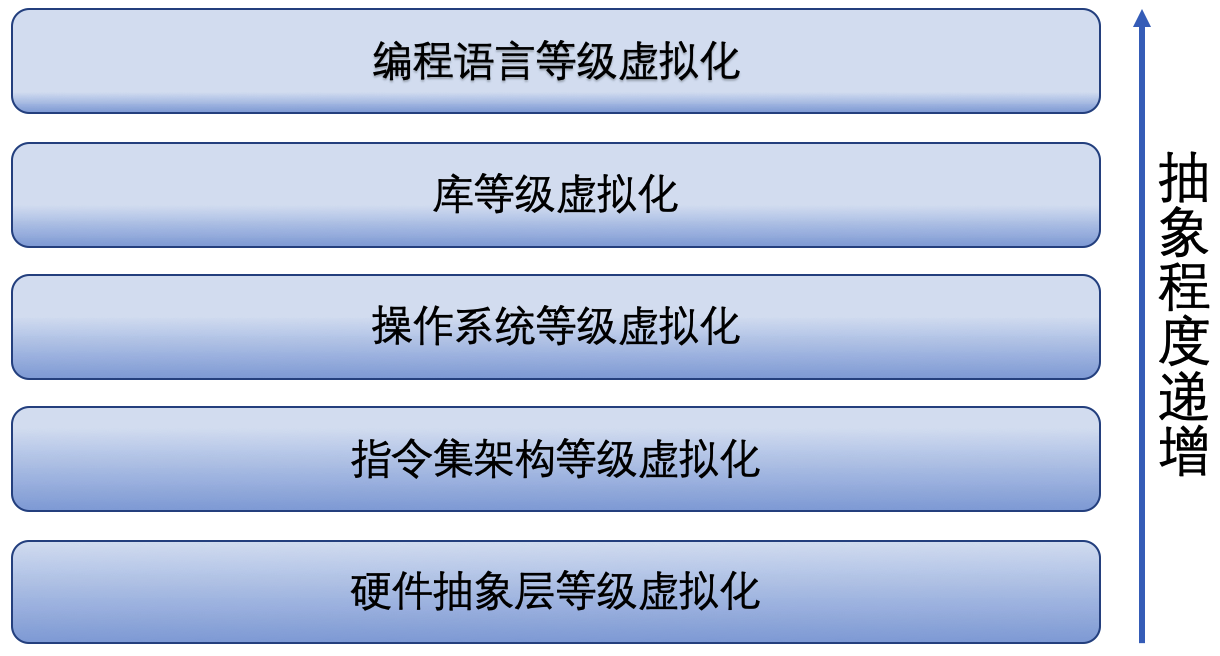
\includegraphics{./Figure/IMG_Chap2_1.png}
  \caption{虚拟技术按抽象程度来分为五个层次}\label{Fig:chap2_1}
\end{figure}

\subsection{虚拟机监视器}
Hypervisor,又称虚拟机器监视器(virtual machine monitor,缩写为 VMM),是用来建立与执行虚拟机器的软件、固件或硬件。

被Hypervisor用来执行一个或多个虚拟机器的电脑称为主体机器(host machine),这些虚拟机器则称为客体机器(guest machine)。hypervisor提供虚拟的作业平台来执行客体操作系统(guest operating systems),负责管理其他客体操作系统的执行阶段;这些客体操作系统,共同分享虚拟化后的硬件资源。

Gerald J.Popek和Robert P.Goldberg 在他们1974年的文章“Formal Requirements for Virtualizable Third Generation Architectures” 发表了两种类型的Hypervisor,分别是类型I和类型II\cite{Kudinskas}。

\textbf{类型I:本地或裸机Hypervisor}

这种虚拟机管理程序直接运行在主机的硬件上,这样便可以直接控制硬件同时对客体操作系统进行管理。

特点:
\begin{enumerate}
    \item 需要硬件支持
    \item 虚拟机监视器作为主操作系统
    \item 运行效率高
\end{enumerate}

举例:
\begin{enumerate}
    \item VMware5.5及以后版本
    \item Xen3.0以后版本
    \item Virtual PC 2005
    \item KVM
\end{enumerate}

\begin{figure}[htbp]
  \centering
  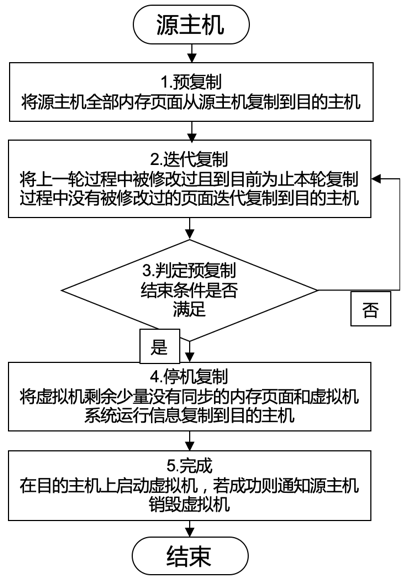
\includegraphics{./Figure/IMG_Chap2_2.png}
  \caption{VMM-Type1}\label{Fig:chap2_2}
\end{figure}

\textbf{类型II:Hosted Hypervisor}

这种虚拟机管理程序运行在主机的操作系统上,跟其他计算机程序没有明显的区别。

特点:
\begin{enumerate}
    \item 虚拟机监视器作为应用程序运行在主操作系统环境内
    \item 运行效率一般较类型I低
\end{enumerate}

举例:
\begin{enumerate}
    \item VMware5.5以前版本
    \item Xen3.0以前版本
    \item Virtual PC 2004
\end{enumerate}

\begin{figure}[htbp]
  \centering
  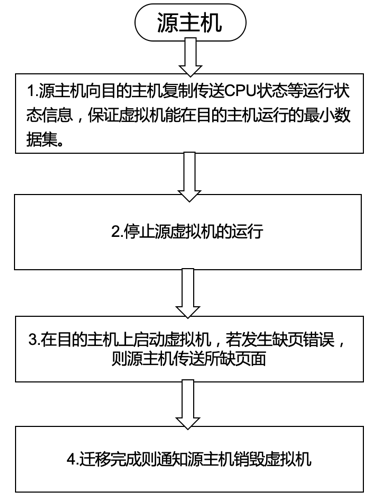
\includegraphics{./Figure/IMG_Chap2_3.png}
  \caption{VMM-Type2}\label{Fig:chap2_3}
\end{figure}

\section{虚拟机动态迁移技术}
最初,纯粹的停机复制方法被用于虚拟机迁移。这包括停止原始虚拟机和在启动新的虚拟机之后,将所有页复制到目标。这个方法的优势在于实现简单但内存迁移需要的时间与虚拟机的内存大小成正比,对于运行服务的实时系统来说,这样的停机时间是不可接受的。

\subsection{虚拟机动态迁移的内容}
虚拟机从一个物理服务器迁移到另一个物理服务器需要迁移到是整个虚拟机的资源和状态。资源主要包括内存、硬盘资源等。状态主要包括运行状态、CPU状态、IO状态、网络状态以及存储状态等。由于不同的资源和状态在虚拟机存在的形式不同,所以要分别针对不同的资源和状态采取不同的迁移方法。

由于CPU具有状态更新快而且数据量不大的特点,所以CPU状态迁移并不会影响到虚拟机迁移的性能,采用Stop-and-Copy方法直接拷贝到目的服务器。

IO状态迁移和CPU状态迁移类似,都可以直接采用停机拷贝的方法,而且不会对虚拟机迁移性能造成影响。

对于网络状态的迁移通常整个数据中心的所有服务器都是在同一个局域网下,那么就可以采用ARP重定向技术。迁移后,源服务器就会将所有数据包传送到目的服务器,从而解决网络状态的迁移问题。
           
一般在大型数据中心集群都会采用共享存储的方式来解决大规模数据存储以及迁移问题。比如分布式文件系统以及网络文件系统等,这样可以大大减少带宽浪费和迁移时间。

内存保存了程序运行过程中的许多重要数据,而且在虚拟机迁移过程中,内存是动态变化的,这对虚拟机迁移提出了更多挑战,是虚拟机动态迁移最难以解决的问题。

内存的迁移一般过程如下:

在预复制内存迁移中,管理程序通常将所有内存页从源复制到目标。当虚拟机仍在源上运行时。如果在此过程中某些内存页发生更改(变为“脏”),它们将继续重新复制,直到重新复制页面的速率不低于页面脏化速率。

在预热虚拟机内存迁移阶段,管理程序将所有内存页从源复制到目标。当虚拟机仍在源上运行时。如果某些内存页在内存复制过程中发生更改,则会变脏。翻页后,将重新复制,直到重新复制的页数不低于页脏率。

在预热阶段之后,虚拟机将在原始主机上停止,剩余的脏页将复制到目标,然后在目标主机上恢复虚拟机。之间的时间间隔在原始主机上停止虚拟机并在目标上恢复虚拟机被称为“停机时间”,范围为根据内存大小和在虚拟机上运行的应用程序数毫秒到秒。有一些减少迁移停机时间的技术,例如使用内存的概率密度函数改变。

\subsection{虚拟机动态迁移的过程}
虚拟机动态迁移的过程主要是内存迁移的过程,内存迁移主要有两种方法:Pre-copy算法和Post-copy算法\cite{Aidan}。

Pre-copy算法的过程:

\begin{figure}[htbp]
  \centering
  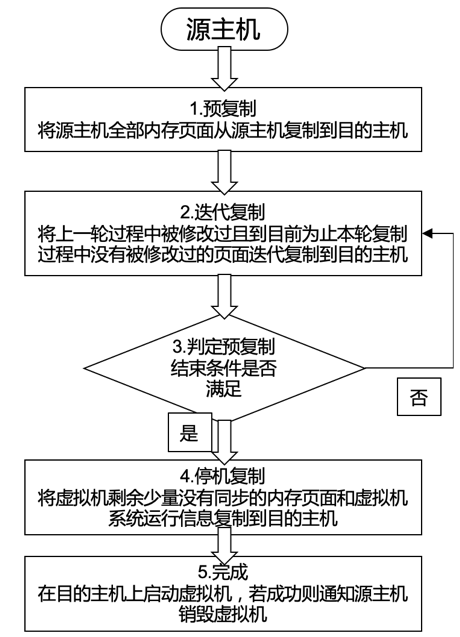
\includegraphics{./Figure/IMG_Chap2_4.png}
  \caption{Pre-copy算法}\label{Fig:chap2_4}
\end{figure}

优点:同静态复制算法相比,Pre-copy算法缩短了停机时间。

不足:负载较高时,内存页面修改频繁,受网络带宽等因素影响,迭代无法收敛进入强制复制阶段,会造成较大的系统开销,引起较长的停机时间和总迁移时间。

Post-copy算法的过程:

\begin{figure}[htbp]
  \centering
  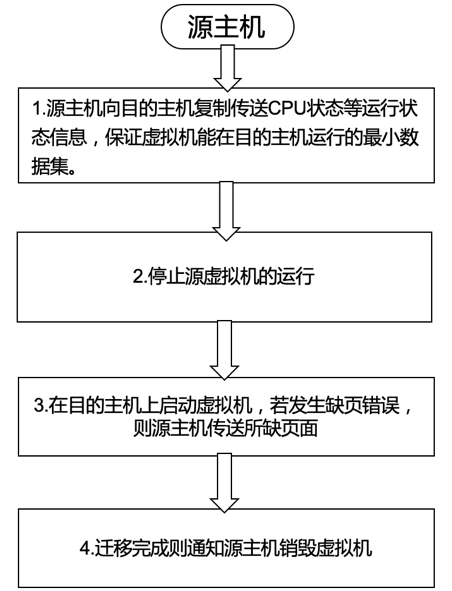
\includegraphics{./Figure/IMG_Chap2_5.png}
  \caption{Post-copy算法}\label{Fig:chap2_5}
\end{figure}

优点:较Pre-copy迁移时间短。

不足:Pull的初始阶段性能较差。算法不稳定,如果迁移途中,目的主机崩溃,则虚拟机数据不可恢复。

\section{蚁群算法}
蚁群算法(Ant Colony Optimization, ACO),又称蚂蚁算法,是一种用来在图中寻找优化路径的概率型优化算法。其灵感来源于蚂蚁在寻找食物过程中发现路径的行为\cite{Maniezzo}。

在蚁群算法中,我们将搜索活动分布在所谓的“蚂蚁”上,即具有非常简单的基本能力的代理,这些能力在某种程度上模仿真实蚂蚁的行为。蚂蚁用于在个体之间就路径传递信息并用于决定去哪里的信息由信息素路径组成。移动的蚂蚁在地面上放置一些信息素(数量不等),从而通过这种物质的痕迹标记出路径。虽然孤立的蚂蚁基本上随机移动,但是遇到先前铺设的蚂蚁的蚂蚁可以检测到它并且很有可能决定跟随它,从而用自己的信息素加强踪迹。出现的集体行为是一种自动催化行为,其中蚂蚁追踪的越多,追踪就越有吸引力。因此,该过程的特征在于正反馈回路,其中蚂蚁选择路径的概率随着先前选择相同路径的蚂蚁的数量而增加。

如图 \ref{Fig:chap2_6} 中所示的实验设置。存在蚂蚁行走的路径(例如从食物源A到巢E,反之亦然)。在路径上放置障碍物,阻断蚂蚁的行走路线。因此,在B位置,蚂蚁必须决定是向左还是向左转。选择受前蚂蚁留下的信息素痕迹强度的影响。在正确的路径上更高水平的信息素使蚂蚁具有更强的刺激,因此更有可能向右转。由于在两个路径上没有先前的信息素,到达B点(或D点)的第一个蚂蚁具有相同的向右或向左转的概率。因为路径BCD比BHD短,所以跟随它的第一只蚂蚁将在路径BHD之后的第一只蚂蚁之前到达D。结果是从E到D返回的蚂蚁将在路径DCB上找到更强的路径,这是由于偶然决定通过DCBA接近障碍的所有蚂蚁的一半以及通过BCD来到的已经到达的蚂蚁:他们将因此,优选(概率上)路径DCB到路径DHB。因此,每单位时间后路径BCD之后的蚂蚁数量将高于BHD之后的蚂蚁数量。这导致较短路径上的信息素数量比较长路径上的信息素数量增长得更快,因此任何单个蚂蚁选择路径遵循的概率很快偏向较短路径。最终的结果是,所有蚂蚁很快就会选择较短的路径。

\begin{figure}[htbp]
  \centering
  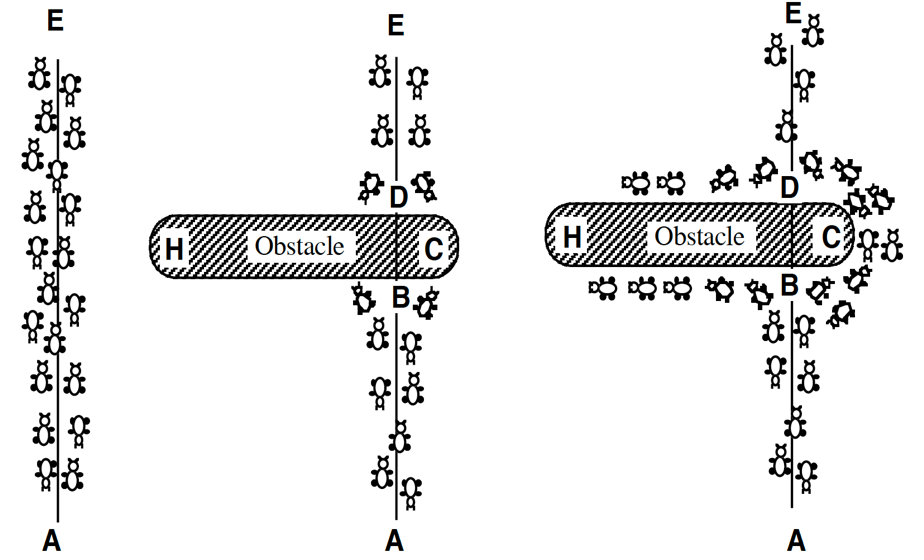
\includegraphics{./Figure/IMG_Chap2_6.png}
  \caption{蚁群算法}\label{Fig:chap2_6}
\end{figure}

\section{本章小结}
本章主要研究了虚拟化技术、虚拟机动态迁移技术以及本文主要采用的蚁群算法的主要思想,为后续的迁移框架设计奠定了基础。

\chapter{面向负载均衡的虚拟机动态迁移框架设计}

\section{总体设计}
本文根据蚁群算法设计了一种面向负载均衡的虚拟机动态迁移框架,在一个数据中心的所有服务器中都部署有该动态迁移模块。服务器可以通过该框架决定何时进行虚拟机的迁移,如何选择服务器中的虚拟机进行迁移以及如何选择迁移的目标服务器等。智能蚂蚁作为服务器间的通信媒介起到了重要的作用,它不但能够记录相关服务器的信息以便于后续的迁移决策而且还能按照一定的规律智能地选择合适的服务器进行搜索,有效提高虚拟机迁移的效率以及通过虚拟机迁移后整个数据中心的负载均衡程度。整体的数据中心互联视图如图 \ref{Fig:chap3_1} 所示。

\begin{figure}[htbp]
  \centering
  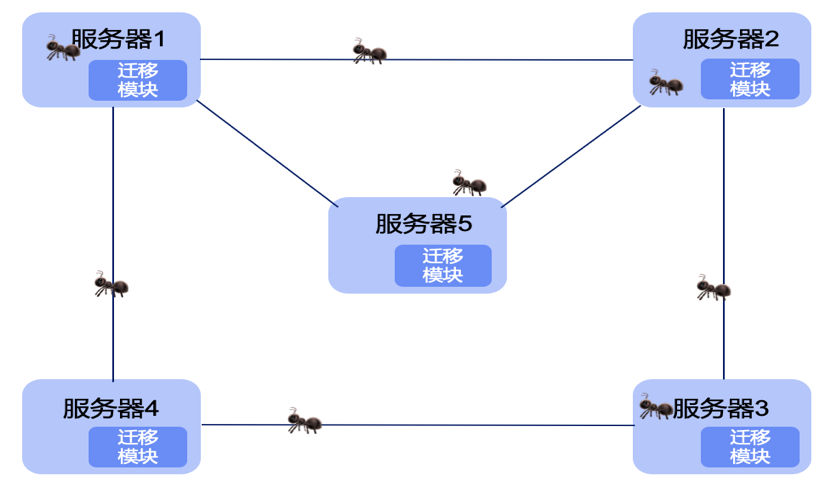
\includegraphics{./Figure/IMG_Chap3_1.png}
  \caption{数据中心互联视图}\label{Fig:chap3_1}
\end{figure}

\section{模块设计}
整个动态迁移框架主要包括以下几个模块:蚂蚁服务模块、蚂蚁算法模块、负载模块、决策模块以及配置库等。框架的体系结构如图 \ref{Fig:chap3_2} 所示。

\begin{figure}[htbp]
  \centering
  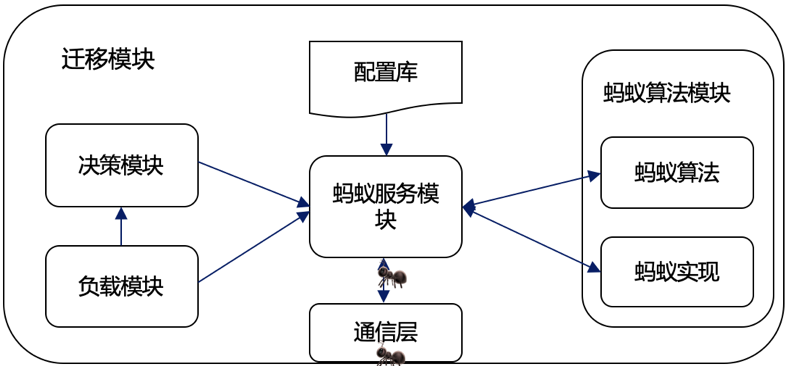
\includegraphics{./Figure/IMG_Chap3_2.png}
  \caption{虚拟机动态迁移框架的体系结构}\label{Fig:chap3_2}
\end{figure}

整个框架体系结构中最重要的就是蚂蚁算法模块。其中蚂蚁算法模块又分为两个部分,蚂蚁的实现以及真正的蚂蚁算法的实现。每个蚂蚁都有一块特定的内存空间,内存空间中主要维护着几个服务器列表。负载列表中记录着蚂蚁搜索过的所有服务器的信息,低负载列表中记录着负载较低的服务器信息,还有一个允许蚂蚁搜索的服务器列表中记录着蚂蚁未经过的服务器信息。其中低负载列表中记录的服务器就是为将来虚拟机迁移的目的服务器提供决策信息。蚂蚁算法的实现主要是对蚂蚁的搜索过程的算法实现。配置库中主要是对迁移框架中的一些重要参数进行配置,比如蚂蚁的步长、虚拟机的状态域阙值的定义、算法的相关参数、每个服务器上的信息素的初始化浓度以及信息素的挥发速率等信息。决策模块主要分为两部分的决策,一部分是选择策略的实现,另一部分是对迁移策略的实现。选择策略主要是在待迁移的服务器上选择需要迁移的虚拟机的策略,迁移策略主要是虚拟机需要迁移到的目的虚拟机的选择策略。负载模块主要是对服务器负载信息的计算方式,来动态判断服务器所处的状态域以便进行迁移决策。蚂蚁服务模块则是对整个虚拟机动态迁移框架进行整合协调与调度,确保框架的各个模块有序地运行。

\subsection{蚂蚁服务模块}
蚂蚁服务模块负责与其他模块进行交互,对整个虚拟机动态迁移框架进行整合协调与调度,确保框架的各个模块有序地运行。蚂蚁服务模块的主要功能如图 \ref{Fig:chap3_3} 所示。

\begin{figure}[htbp]
  \centering
  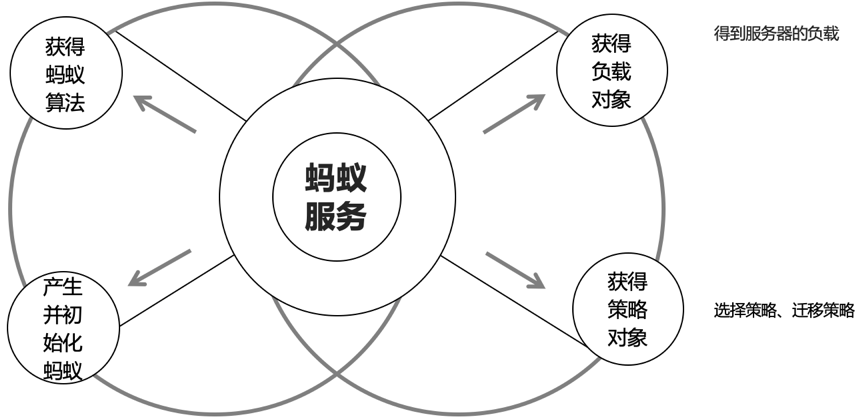
\includegraphics{./Figure/IMG_Chap3_3.png}
  \caption{蚂蚁服务模块}\label{Fig:chap3_3}
\end{figure}

\subsection{蚂蚁的产生及初始化}
根据服务的负载值,本文设计了一个服务器负载域状态模型,将服务器的负载分为四个状态域:低负载域、平衡域、过载域和超载域。如图 \ref{Fig:chap3_4} 所示。

\begin{figure}[htbp]
  \centering
  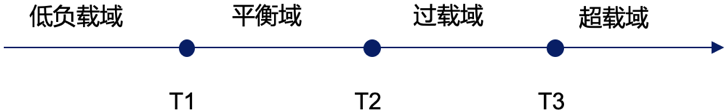
\includegraphics{./Figure/IMG_Chap3_4.png}
  \caption{服务器负载状态域模型}\label{Fig:chap3_4}
\end{figure}

其中$ T1 $为平衡域阈值,$ T2 $为过载域阈值,$ T3 $为超载域阈值,当服务器处于超载域时,产生搜索蚂蚁并进行虚拟机迁移。

服务器在运行过程中会不断计算自己的负载值来动态判断所处的状态域,当服务器的负载值超过超载域阙值$ T3 $时表示服务器已经超载,这时服务器会产生蚂蚁,蚂蚁负责在数据中心中搜索低负载的服务器并将相应的服务器信息记录到蚂蚁内存的低负载列表中。这样在蚂蚁搜索完毕后(即蚂蚁的步长为0时)会根据蚂蚁内存中低负载列表的服务器信息按照迁移策略进行迁移目标服务器的选择。在蚂蚁产生之后进行初始化操作,首先初始化蚂蚁的步长,步长决定了蚂蚁在数据中心服务器集群中搜索的距离。所以蚂蚁的步长应该根据数据中心整体的负载均衡程度进行调整。接下来初始化负载列表、低负载列表以及蚂蚁未经过的服务器列表,蚂蚁未经过的服务器列表默认为该数据中心全部的服务器。蚂蚁每经过一个服务器就会将服务器加入负载列表,防止蚂蚁进行重复的搜索,并将服务器从蚂蚁未经过的服务器列表中删除,而且会检测每一个经过的服务器的的负载均衡值,如果该服务器的负载值处于低负载域,那么就将该服务器的信息加入到低负载列表中。蚂蚁就按照这样的方式进行搜索直达蚂蚁的步长为0,搜索完成后,首先从待迁移的服务器中选择需要迁移的虚拟机,然后根据蚂蚁内存中记录的低负载的服务器列表从其中选择合适的服务器进行虚拟机迁移操作。

\subsection{蚂蚁实体及蚂蚁算法}
蚂蚁作为数据中心各个服务器间的通信媒介,担负着搜索并记录服务器信息的重要作用,并且为之后虚拟机的迁移策略提供重要的信息,蚂蚁实体的相关实现如下代码所示。

\begin{lstlisting}[language=C,caption={蚂蚁实体},label=Code:java]
public class Ant {

    // 蚂蚁剩余步数
    private int remanentSteps;

    // 负载列表中记录着蚂蚁搜索过的所有服务器的负载信息
    private List<Server> loadList;

    // 低负载列表中记录着负载较低的服务器信息
    private List<Server> underLoadedList;

    // 蚂蚁未经过的服务器
    private List<Server> allowedList;

    private Server currentServer;

    // 蚂蚁的初始化
    public void initAnt(Server server) {
            
        }

    // 选择蚂蚁下一个要搜索的服务器
    public Server selectNextServer() {

       // 概率矩阵
        List<Float> pList = new ArrayList<>();

        Datacenter datacenter = currentServer.getDatacenter();
        List<Server> serverList = datacenter.getHostList();
        for (Server server : serverList) {
             boolean flag = false;

             // 计算概率矩阵
            for (Server server1 : allowedList) {
                if (server.getId() == server1.getId()) {
                    pList.set(server.getId(), 
                    (float) (Math.pow(1 / server.getPheromone(), CommonConfig.alpha) *
                             Math.pow(server.getBw(), CommonConfig.beta) *
                             Math.pow(1 - server.getLoad(), CommonConfig.rho) / sum));

                    break;
                }
            }
        }

        // 轮盘赌选择下一个服务器
        Random random = new Random(System.currentTimeMillis());
        float selectP = random.nextFloat();
        float sumP = 0;
        Server selectServer = null;
        for (Server server : serverList) {
            sumP += pList.get(server.getId());
            if (sumP >= selectP) {
                selectServer = server;
                break;
            }
        }

        allowedList.remove(selectServer);
        loadList.add(selectServer);
        currentServer = selectServer;
        return selectServer;
    }
}
\end{lstlisting}

我们前面已经详细论述了蚂蚁内存空间的相关服务器列表及其初始化,蚂蚁实体中还有一个重要的功能就是自己按照一定的算法去选择下一个要搜索的服务器。蚂蚁搜索下一个目标服务器时并不是毫无目的地寻找,而是根据一定的信息按照一定的概率去搜索。本文根据数据中心服务器的相关特点综合考虑了蚂蚁在选择下一个要搜索的服务器时所要考虑的因素。除了信息素的浓度之外,还要根据服务器的负载值以及服务器的网络状态信息等因素综合选择蚂蚁下一个要搜索的服务器。在蚁群算法当中,信息素浓度越高,蚂蚁选择该条路径的概率就越大。在本文的应用场景当中,还是借鉴这种思想,蚂蚁频繁搜索的服务器应该是负载较低的服务器,那么蚂蚁留下的信息素浓度就会越大,相应的服务器上的信息素的浓度就会高于负载较高的服务器,那么后续蚂蚁也会大概率选择这些服务器。除此之外服务器的负载值和网络状况也是重要的考虑因素。服务器的负载值高,表明服务器需要进行虚拟机迁移操作,那么蚂蚁应该避免搜索负载值高的服务器,负载值越低,蚂蚁搜索该服务器的概率越大。另外蚂蚁因该优先选择服务器剩余带宽较大的服务器,以便于提高虚拟机迁移的效率。所以综合以上考虑的因素,最终根据概率选择蚂蚁需要搜索的下一个服务器。根据蚁群算法的相关知识,蚂蚁在 i 节点选择 j 节点的概率如下公式所示。

\begin{figure}[htbp]
  \centering
  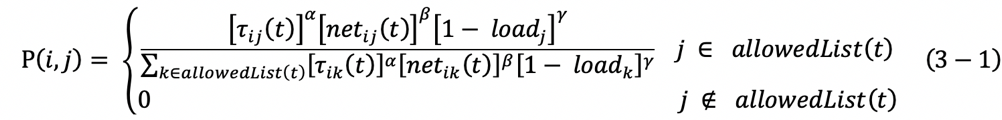
\includegraphics[width=0.8\linewidth]{./Figure/IMG_Chap3_5.png}
\end{figure}

$ τ_{ij} (t) $表示节点$ i $观察到的节点$ j $的信息素浓度,$allowedList(t) $表示$ t $时刻蚂蚁可以访问的服务器列表,蚂蚁每经过一个服务器就将该服务器从允许列表中移除以防止进行重复搜索,$net_{ij} (t) $标记服务器$ i $和服务器$ j $之间带宽的影响,带宽越大,服务器被选择的概率越大,$1 - load_j $表示节点的负载值越低,那么$ 1 - load_j $的值越大,服务器被选择的概率越大。$ α、β、γ $体现了信息素浓度、网络状态和负载值在服务器选择中的相对重要性,其中$ α ≥0,β ≥0,γ ≥0 $。

蚂蚁算法的核心主要是根据蚂蚁的步长以及蚂蚁对蚂蚁对服务器的选择进行搜索,在搜索过程中根据服务器的负载值判断服务器所处的负载域,如果蚂蚁搜索的服务器处于低负载域,则把相应的服务器信息记录到蚂蚁内存中对应的低负载列表中。最后对服务器的信息素进行更新。蚂蚁算法的实现如下代码所示。

\begin{lstlisting}[language=C,caption={蚂蚁算法},label=Code:java]
public class AntAlgorithm {

    public void doSearchServer(Ant ant) {

        for (int step = CommonConfig.steps; step > 0; step--) {
            Server server = ant.selectNextServer();

            if (server.getLoad() <= CommonConfig.threshold1) {
                ant.getUnderLoadedList().add(server);
            }

            Datacenter datacenter = server.getDatacenter();
            List<Server> serverList = datacenter.getHostList();
            // 信息素挥发
            for (Server ser : serverList) {
                server.setPheromone(ser.getPheromone() * (1 - CommonConfig.rate));
            }
            // 信息素更新
            server.setPheromone(server.getPheromone() + CommonConfig.base * (1 - server.getLoad()));
        }
    }
}
\end{lstlisting}

为了及时反应信息素的变化,在蚂蚁搜索服务器的过程中会实时地更新服务器的信息素浓度。全局信息素更新方式如下公式所示。

\begin{figure}[htbp]
  \centering
  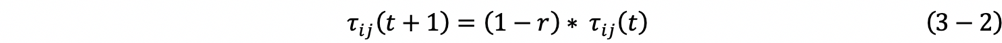
\includegraphics[width=0.3\linewidth]{./Figure/IMG_Chap3_6.png}
\end{figure}

其中$ r $是全局信息素挥发速率,且$ 0 < r < 1$。

\subsection{服务器负载计算}
 服务器的负载值是衡量一个服务器运行状态和负载均衡状况的重要指标,也是进行虚拟机迁移的重要参考,本文还会根据服务器的负载值动态的标记服务器所处的负载域。计算一个服务器负载值所需要考虑的因素有很多,本文根据服务器的三种资源来计算服务器的负载值:CPU、内存和带宽。定义的服务器负载值的计算方式如下。

 \begin{figure}[htbp]
  \centering
  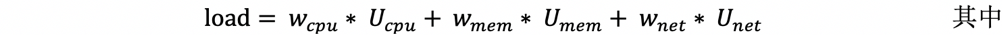
\includegraphics[width=0.3\linewidth]{./Figure/IMG_Chap3_7.png}
\end{figure}

 \begin{figure}[ht]
  \centering
  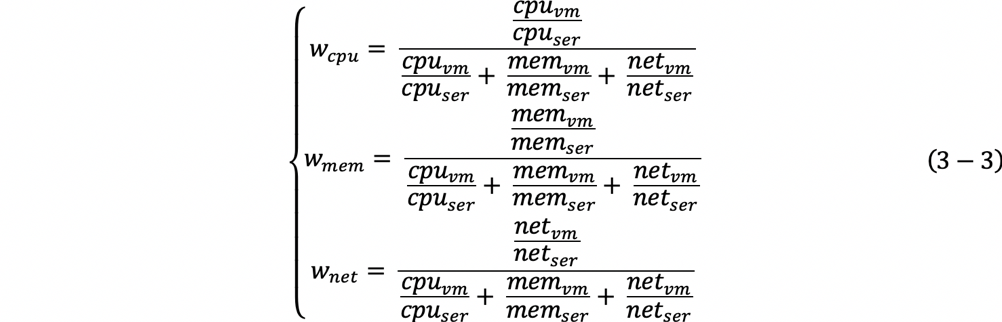
\includegraphics[width=0.3\linewidth]{./Figure/IMG_Chap3_8.png}
\end{figure}

$ w_{cpu} $、$ w_{mem} $、$ w_{net} $分别代表服务器的CPU、内存和带宽所占的权重。$ U_{cpu} $、$ U_{mem} $、$ U_{net} $则分别代表服务器CPU 的利用率,服务器内存的利用率以及服务器带宽的利用率。$ load $代表服务器的负载值,反映了服务器运行状态和负载均衡状况。

\section{相关策略}
蚂蚁在完成对数据中心的服务器搜索之后,蚂蚁内存中的低负载列表记录着低负载的迁移目标服务器列表。接下来在进行虚拟机迁移之前还需要解决两个问题。一是在需要虚拟机迁移的服务器上选择一台合适的虚拟机进行迁移,二是在蚂蚁内存中的低负载列表记录的迁移目标服务器列表选择一台服务器进行迁移。前者本文称作待迁移虚拟机的选择策略,后者本文称作目标服务器的迁移匹配策略。

\subsection{待迁移虚拟机的选择策略}
现在已有的待迁移虚拟机的选择策略,比如选择迁移所需时间最短的虚拟机,选择资源利用率最低的虚拟机或者随机选择虚拟机。这些选择策略考虑的因素的过于单一,不能充分满足虚拟机迁移的各方面的要求。所以本文打算综合考虑虚拟机的资源利用率以及虚拟机迁移成本等因素,即在尽量选择负载值较高的服务器的同时降低虚拟机迁移的成本。

首先要确定使服务器负载过高的因素,常见的考虑因素主要有CPU、内存及带宽,那么就要计算三种因素各自所占用的比例,计算公式如下。

 \begin{figure}[htbp]
  \centering
  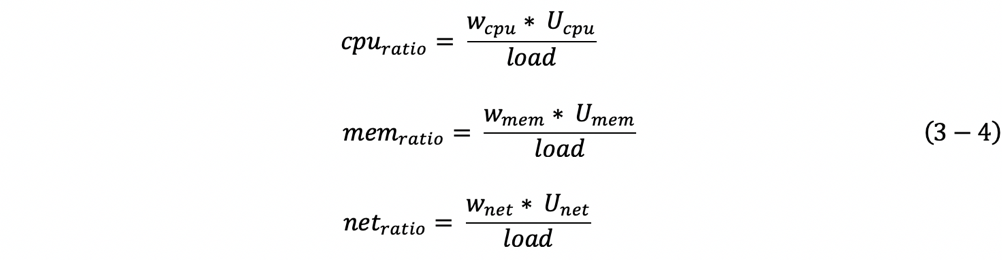
\includegraphics[width=0.3\linewidth]{./Figure/IMG_Chap3_9.png}
\end{figure}

 \begin{figure}[htbp]
  \centering
  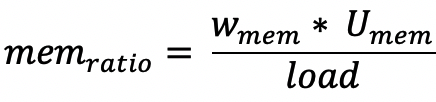
\includegraphics[width=0.3\linewidth]{./Figure/IMG_Chap3_10.png}
\end{figure}

 \begin{figure}[htbp]
  \centering
  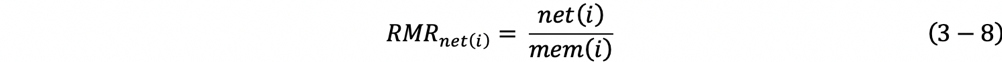
\includegraphics[width=0.3\linewidth]{./Figure/IMG_Chap3_11.png}
\end{figure}

计算得到值最大的即为导致服务器负载过高的决定的因素,然后根据这一因素决定需要迁移的虚拟机。为了同时考虑虚拟机迁移成本,还要考虑虚拟机占用的内存空间,那么就需要计算服务器的各个虚拟机的瓶颈资源和虚拟机占用内存的比值。定义变量RMR来表示使服务器负载过高的瓶颈资源与虚拟机占用内存的比值。按照使虚拟机负载过高的瓶颈资源不同的选择方式如下。

\begin{enumerate}[(1)]
    \item 如果CPU是使服务器负载过高的瓶颈资源,那么按照如下公式计算服务器每个虚拟机的RMR。

     \begin{figure}[htbp]
      \centering
      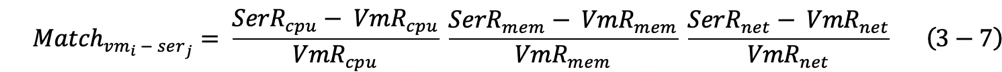
\includegraphics[width=0.3\linewidth]{./Figure/IMG_Chap3_12.png}
    \end{figure}

      其中$ VmU_{cpu(i)} $表示虚拟机的CPU利用率,$VmU_{mem(i)} $表示虚拟机占用服务器的内存比例。那么最后选择RMR的值最大的虚拟机作为待迁移的虚拟机。
    \item 如果内存使服务器负载过高的瓶颈资源。那么选择占用内存最大的虚拟机作为待迁移的虚拟机。
    \item 如果带宽是使服务器负载过高的瓶颈资源,那么按照如下公式计算服务器每个虚拟机的RMR。

    \begin{figure}[htbp]
      \centering
      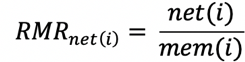
\includegraphics[width=0.3\linewidth]{./Figure/IMG_Chap3_13.png}
    \end{figure}

    其中 $ net(i) $表示虚拟机的占用带宽,$ mem(i) $表示虚拟机占用的内存。那么最后选择RMR的值最大的虚拟机作为待迁移的虚拟机。
\end{enumerate}

\subsection{目标服务器的迁移匹配策略}
蚂蚁在完成对数据中心的服务器搜索之后,需要在蚂蚁内存中的低负载列表记录的迁移目标服务器列表选择一台服务器进行迁移。为了解决待迁移虚拟机需求资源和服务器剩余资源之间的匹配的问题,本文定义的一种匹配度$ Match_{vm-ser} $的概念,公式如下所示。

\begin{figure}[htbp]
  \centering
  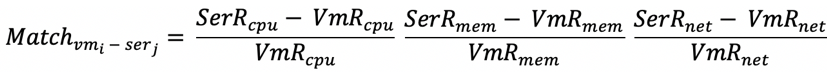
\includegraphics[width=0.8\linewidth]{./Figure/IMG_Chap3_14.png}
\end{figure}

其中,$ SerR_{cpu} $、$ SerR_{mem} $、$ SerR_{net} $分别代表服务器剩余的CPU、内存和带宽资源。$ VmR_{cpu} $、$ VmR_{mem} $、$ VmR_{net} $则分别代表虚拟机需要的CPU、内存和带宽资源。如果$ Match_{vm_i-ser_j} < 0 $则说明待迁移虚拟机与该目标服务器匹配失败,即虚拟机需要的资源超过了服务器的剩余资源。

待迁移虚拟机与目标服务器列表的匹配过程如下。
\begin{enumerate}[(1)]
    \item 从蚂蚁内存的低负载服务器列表中获取迁移目标服务器。
    \item 依次遍历每一个服务器计算其匹配度。
    \item 对服务器的匹配度进行排序,取匹配度最大的服务器作为虚拟机迁移的目标服务器。
    \item 若所有的服务器的匹配度均小于 0 ,则该服务器重新生成蚂蚁开始下一轮搜索过程。
    \item 开始虚拟机迁移。
\end{enumerate}

\section{本章小结}
本章主要介绍了面向负载均衡的虚拟机动态迁移框架的设计,首先从整体上介绍了该框架在服务器上所处的位置以及所起到的作用。然后详细地介绍了该动态迁移框架的各个模块的设计。最后介绍了待迁移虚拟机的选择策略和目标服务器的迁移匹配策略。整个框架的设计基本如前所述,本章都做了详细介绍。

\chapter{仿真实验与结果分析}
本章将对本文提出的面向负载均衡的虚拟机动态迁移框架进行仿真实验,借助 CloudSim 这个云计算模拟框架,仿真云计算环境下的数据中心、服务器以及虚拟机等云计算基础设施,并应用本文提出的虚拟机迁移框架进行虚拟机迁移的模拟,最终对这个虚拟机迁移框架的性能及其最终的负载均衡效果进行分析与评估。

\section{CloudSim 介绍}
云计算是IT基础设施和应用程序作为在基于使用的支付模式下向最终用户提供“服务”。它甚至可以利用虚拟化服务根据随时间变化的需求运行。评估云资源调配策略、应用程序工作负载模型的性能等要求很难实现。为了解决这个问题,一个可扩展的支持云计算系统和应用程序建模和仿真的仿真工具 CloudSim 应运而生\cite{Atanasov}。目前,它支持云计算环境的建模和仿真,包括单网络云和网络间云(云的联合)。此外,它还公开了网络间云下虚拟机分配的实施策略和配置技术的计算场景。

CloudSim 的核心架构如图 \ref{Fig:chap4_1} 所示。

\begin{figure}[htbp]
  \centering
  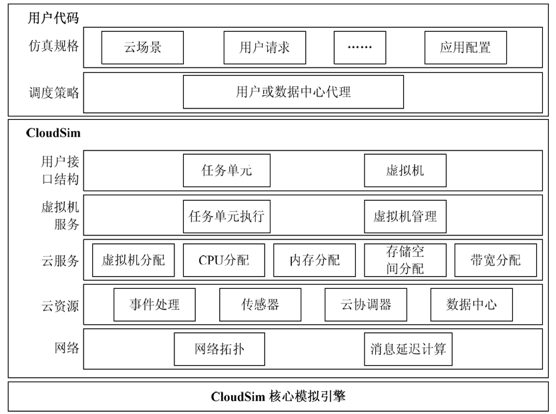
\includegraphics{./Figure/IMG_Chap4_1.png}
  \caption{CloudSim 的核心架构}\label{Fig:chap4_1}
\end{figure}

 CloudSim仿真层支持基于云的虚拟化数据中心环境的建模和仿真,包括用于虚拟机的专用管理接口。对于一些基本问题,如向虚拟机提供主机,管理应用程序执行和监视动态系统状态都由这一层处理。一个云提供商,他想研究不同策略在将其主机分配到虚拟机,需要在这一层实现他的策略。这样的实施可以通过编程扩展核心虚拟机分配功能来完成。总之,通过 CloudSim,研究人员将能够根据特定的场景和配置执行测试,从而允许在与云相关的所有关键方面进行最佳实践计算。

 \section{实验环境搭建}
云数据中心不断的运转,各个实体(Vm,Host等)每时每刻的状态都在变化,CloudSim 通过基于事件的机制对数据中心各个实体的状态变化进行模拟。数据中心与数据中心代理之间的事件传递过程如图 \ref{Fig:chap4_2} 所示。

\begin{figure}[htbp]
  \centering
  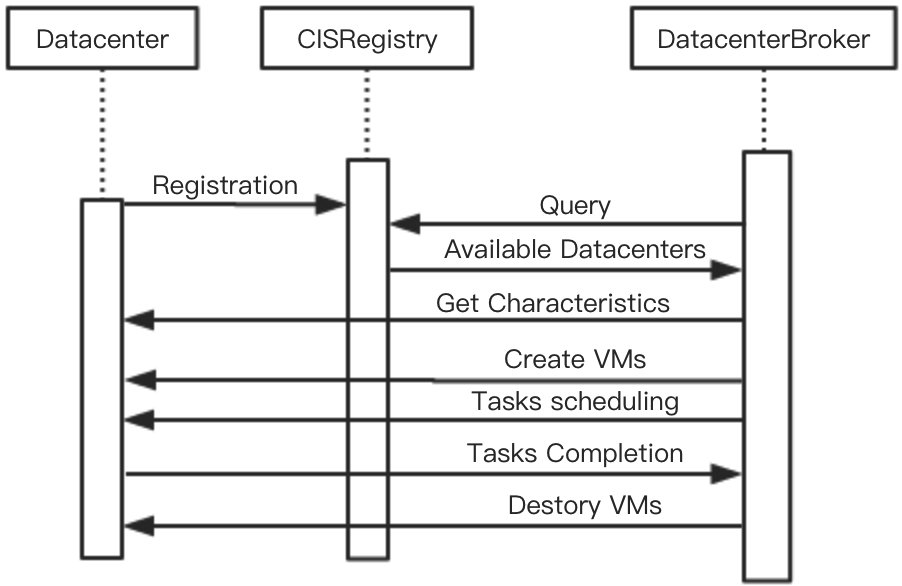
\includegraphics{./Figure/IMG_Chap4_2.png}
  \caption{事件传递机制}\label{Fig:chap4_2}
\end{figure}

每个数据中心实体在 CIS 注册表中注册。然后,CIS提供信息注册表类型的功能。首先数据中心和数据中心代理之间往来事件以确认DataCenterCharacteristic创建完成,然后Br数据中心代理产生事件要求数据中心创建虚拟机,虚拟机创建完毕后,数据中心代理接着产生云任务提交事件要求数据中心处理分配的云任务,数据中心调用相关函数更新集群状态(相当于执行任务)、最终产生任务完成事件,数据中心代理发出销毁虚拟机事件,模拟过程基本结束。

数据中心执行任务的过程也稍显复杂,任务单元的处理由各自的虚拟机处理.因此,必须在每个模拟步骤中不断更新和监控任务单元的进度。在每个模拟步骤中,每个数据中心实体都为其管理的每个主机调用一个名为updateVmsProcessing()的方法。在此之后,当前的已联系的vms更新处理主机的活动任务。此方法的输入参数类型是当前模拟时间,返回参数类型是当前正在运行的任务的下一个预期完成时间.在主机级别,调用updateVMsprocessing()会触发updateCloudletsprocessing()方法,该方法指示每个VM更新其任务单元状态(完成、挂起、执行)数据中心实体。此方法实现了与前面针对updateVmsProcessing()描述的类似的逻辑,但在VM级别。调用此方法后,vms将返回下一个预期的他们当前管理的任务单元的完成时间。图 \ref{Fig:chap4_3} 以序列图的形式描述了这个过程。

\begin{figure}[htbp]
  \centering
  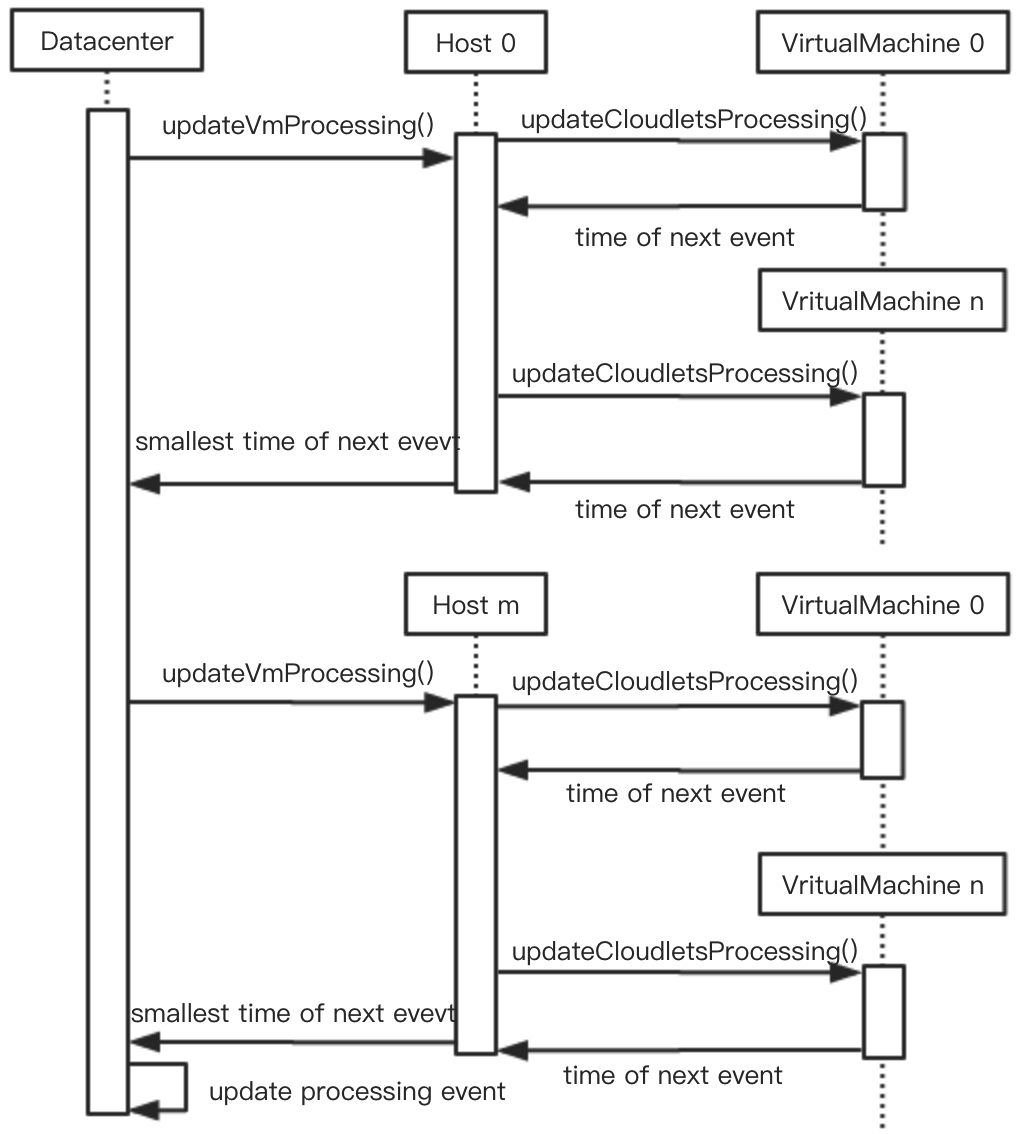
\includegraphics{./Figure/IMG_Chap4_3.png}
  \caption{任务执行过程}\label{Fig:chap4_3}
\end{figure}

根据以上对 CloudSim 模拟过程的分析,找到了将本文设计的虚拟机迁移框架与 CloudSim 进行接入的切入点。在 CloudSim 中有两个有关于虚拟机迁移的重要的抽象类:PowerVmSelectionPolicy 和 PowerVmAllocationPolicyMigrationAbstract。前者中有一个重要的抽象方法 getVmToMigrate(PowerHost host),该方法的目的就是从给定的服务器中选择需要迁移的虚拟机,这与本文的待迁移的虚拟机选择策略其实完成的一个功能,那么我们就可以实现 PowerVmSelectionPolicy 的 getVmToMigrate(PowerHost host)方法,将本文的虚拟机动态迁移框架的待迁移的虚拟机选择策略接入。对于 PowerVmAllocationPolicyMigrationAbstract 有两个与虚拟机迁移有关的重要方法:optimizeAllocation()和 isHostOverUtilized(PowerHost powerHost)。前者通过调用后者判断某个服务器是否过载,并为待迁移的虚拟机选择合适的迁移目的服务器,并最终返回一个待迁移的虚拟机迁移目的服务器的映射列表,这样我们可以根据上文所述的目标服务器的迁移匹配策略对上述方法进行重写,实现策略的接入。还有一个重要的类需要进行扩展,那就是服务器对应的类,本文对 PowerHost 类进行扩展,添加一些对于本文对虚拟机迁移框架模拟需要的重要数据,比如服务器的负载值、信息素初始化浓度、蚂蚁服务对象、蚂蚁实体以及策略对象等。还需要添加产生搜索蚂蚁并对其初始化以及对数据中心的搜索方法等。

 \section{实验相关数据}
首先要初始化一个数据中心,假设数据中心等服务器规模为 30 台。影响服务器性能的主要因素有三个:CPU、内存和带宽。同时这三个因素也是初始化一个服务器所必不可少的。
为了实现模拟虚拟机的迁移,假设在前 20 台服务器上分别部署两台虚拟机,在后 10 台服务器上只部署 1 台虚拟机,分别向各个虚拟机提交云任务,使其处于负载状态,可以通过多次改变虚拟机的配置进行多次仿真器实验。设置服务器状态域阙值$ T1 = 0.4,T2 = 0.7,T3 = 0.75 $。在实验的过程中可以动态改变蚂蚁步长,蚂蚁内存空间大小,信息素挥发速率等虚拟机迁移框架的关键参数,比较不同情况下的虚拟机迁移效果以及数据中心整体的负载均衡情况。

 \section{实验结果与分析}
如何衡量本文设计的面向负载均衡的虚拟机迁移框架的负载均衡效果也是本文研究的重要内容。本文提出了一种数据中心负载均衡值的计算方法,公式如下。

\begin{figure}[htbp]
  \centering
  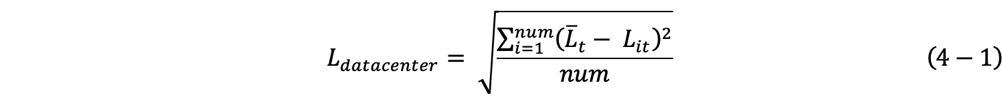
\includegraphics[width=0.3\linewidth]{./Figure/IMG_Chap4_4.png}
\end{figure}

其中,$ num $表示数据中心服务器的数量,$ L_{it} $表示在第$ t $个调度间隔服务器 i 的负载均衡值,$ \overline{L}_t $表示在第$ t $个调度间隔数据中心的平均负载均衡值。$ \overline{L}_t $的定义如下。

\begin{figure}[htbp]
  \centering
  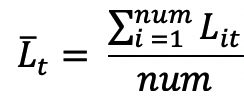
\includegraphics[width=0.3\linewidth]{./Figure/IMG_Chap4_5.png}
\end{figure}

根据以上公式并选取虚拟机迁移框架的几个重要参数进行虚拟机迁移实验,计算实验结果并对实验结果进行评估。
信息素挥发速率$ r $决定了服务器的信息素浓度,首先对信息素挥发速率 r 对虚拟机迁移以及数据中心的负载均衡效果的影响进行实验分析。设置数据中心的调度间隔为 30s,数据中心每次的运行时间为 3600s,共进行 20 次实验。对信息素挥发速率 r 取不同的值,通过上述公式对数据中心的负载均衡值进行计算,得到的结果如表 4-1 所示。

\begin{longtable}[c]{cC{2cm}C{2cm}C{2cm}}
\caption{信息素挥发速率对负载均衡值的影响}\label{Tab:longtable}\\
\hline
初始值 & 负载均衡最优值 & 负载均衡平均值 & 负载均衡最差值\\
\hline
\endfirsthead %以上是最前的表头
\multicolumn{4}{c}{\zihao{4}续表 \thetable\quad 信息素挥发速率对负载均衡值的影响}\\
\hline
初始值 & 负载均衡最优值 & 负载均衡平均值 & 负载均衡最差值\\
\hline
\endhead %以上是换页后的表头,如未换页,并不会显示
\hline
\multicolumn{4}{r}{接下页续表……}\\
\endfoot %以上是前页的表尾,如未换页,并不会显示。
\hline
\endlastfoot%以上选填最后也的表尾。一般不填
%下面开始长表格的内容
0.2 & 0.1824 & 0.2195 & 0.2547\\
0.3 & 0.1543 & 0.1955 & 0.2489\\
0.4 & 0.1234 & 0.1868 & 0.2372\\
0.5 & 0.0971 & 0.1734 & 0.2138\\
0.6 & 0.0709 & 0.1497 & 0.2008\\
0.7 & 0.0968 & 0.1599 & 0.2232\\
0.8 & 0.1279 & 0.1997 & 0.2376\\
0.9 & 0.1854 & 0.2208 & 0.2587\\
\end{longtable}

从表中的数据我们大致可以得到以下结论:随着信息素的挥发速率 r 的初始值不断增大,数据中心的负载均衡值不断减小,当挥发速率的初始值到达一定值时,数据中心的负载均衡值又开始增大。一个合理的解释就是,当信息素的挥发速率过快或过慢时,都会导致数据中心的各个服务器的信息素浓度差异不大,导致蚂蚁在搜索服务器的过程中信息素的浓度对蚂蚁的路径选择作用降低,蚂蚁对信息素浓度的感知不敏感。

除了信息素的挥发速率外,对框架起到重要影响的参数还有蚂蚁的步长。如果蚂蚁的步长过短,可能搜集的低负载服务器信息不足,导致蚂蚁再次搜索,影响虚拟机迁移的效率。如果蚂蚁的步长过长,会导致蚂蚁的搜索时间过长,也同样会影响虚拟机迁移的效率。最终都会影响到数据中心的负载均衡状态。所以我们要找到一个蚂蚁搜索的合适的步长,以及研究蚂蚁的步长对数据中心达到负载均衡的效率的影响。所以根据上文的数据中心的负载均衡值来定义一个数据中心的负载均衡效率公式,如下所示。

\begin{figure}[htbp]
  \centering
  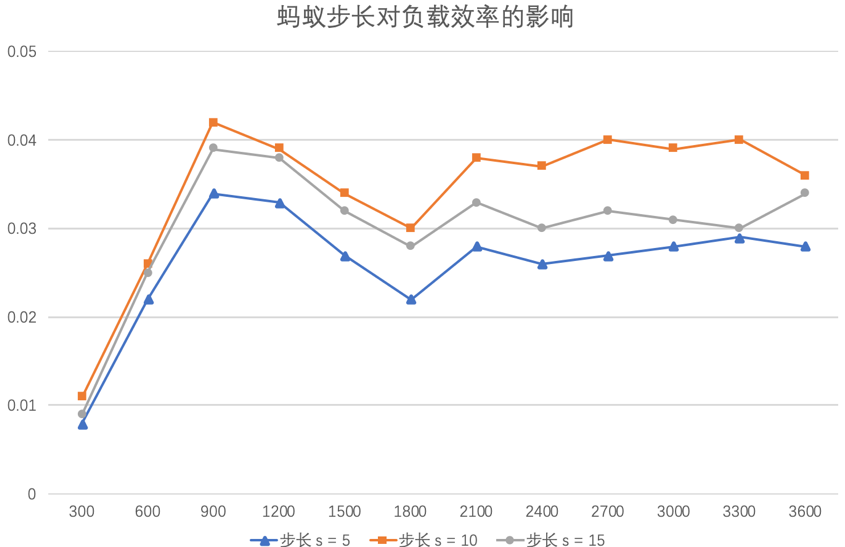
\includegraphics[width=0.3\linewidth]{./Figure/IMG_Chap4_6.png}
\end{figure}

$ T $表示数据中心的负载均衡值达到$ L_T $所花费的时间,$ L_0 $表示数据中心的初始负载均衡值,$ L_T $表示数据中心在$ T $时刻的负载均衡值。设置数据中心的调度时间间隔为 300s,数据中心运行的总时间为 3600s,计算每个调度时间点的$ L_{eff} $,绘制的蚂蚁的步长对数据中心的负载均衡效率的影响统计图如图所示。

\begin{figure}[htbp]
  \centering
  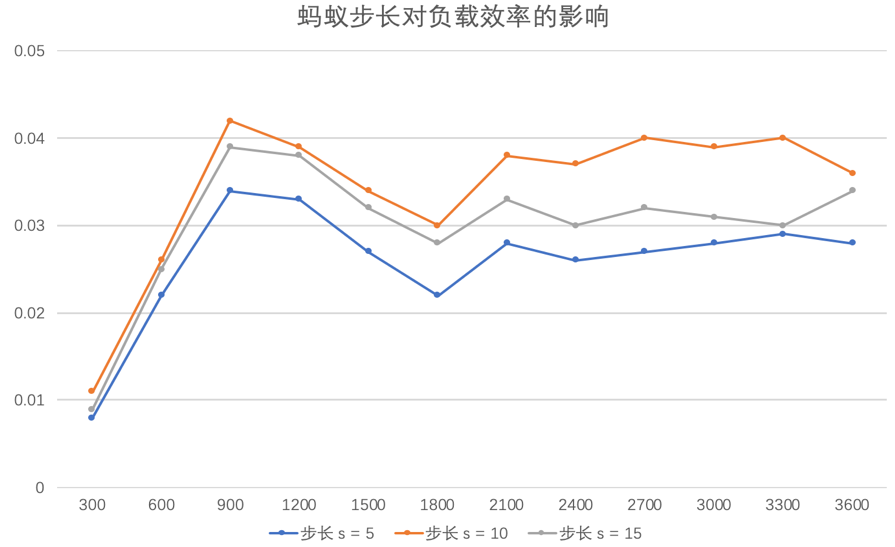
\includegraphics{./Figure/IMG_Chap4_7.png}
\end{figure}

根据上图分析可以得出以下结论:若蚂蚁的步长过短,如步长$ s = 5$,可能搜集的低负载服务器信息不足,导致蚂蚁再次搜索,影响虚拟机迁移的效率。若蚂蚁的步长过长,如$ s = 15 $,会导致蚂蚁的搜索时间过长,也同样会影响虚拟机迁移的效率。当蚂蚁的程度在一个比较合适的值时,比如$ s = 10 $,则在蚂蚁的搜索效率和虚拟机迁移的虚拟机的迁移的效率之间可以找到适当的平衡,使数据中心达到负载均衡的效率达到一个比较高的水平。

 \section{本章小结}
根据上述分析,我们讨论了信息素挥发速率和蚂蚁步长对虚拟机迁移以及数据中心负载均衡的影响,并分别做了相应的分析,但基本可以证明本文设计的虚拟机动态迁移框架还是有一个比较好的负载均衡效果。

\chapter{总结与展望}
本文经过前四章的研究,深入介绍了本文设计的面向负载均衡的虚拟机动态迁移框架并且通过模拟实验对框架的负载均衡效果进行了比较深入的分析,得出了本文设计的虚拟机动态迁移框架具有比较好的负载均衡效果的结论。下面总结一下本文完成的主要工作。

\begin{enumerate}[(1)]
    \item 学习了云计算及虚拟化的相关概念,研究虚拟机动态迁移的技术。
    \item 设计了虚拟机动态迁移框架。借鉴蚁群算法的思想,利用蚂蚁在搜索过程中获取并记录服务器信息,并根据信息素等信息不断优化搜索路径,找到适合迁移的虚拟机。并通过设置不同的阙值来定义一个服务器的负载状态模型,通过定时计算服务器的负载值来动态观察服务器所处的负载域,当服务器过载便会生成蚂蚁去搜寻可以迁移的服务器。最终通过一定的选择策略来选择待迁移服务器上适合迁移的虚拟机,以及一定的迁移策略来选择适合迁移的目的服务器,最终完成虚拟机的迁移过程。
    \item 扩展了云计算模拟平台 CloudSim,仿真云计算环境下的数据中心、服务器以及虚拟机等云计算基础设施,并应用本文提出的虚拟机迁移框架进行虚拟机迁移的模拟,最终对这个虚拟机迁移框架的性能及其最终的负载均衡效果进行了分析与评估。
\end{enumerate}

但是,由于时间以及个人能力的关系,本文的研究工作还有一些不足之处,还有很多可以进行深入研究的方面,主要的方面如下:

\begin{enumerate}[(1)]
    \item 对于服务器的负载可以根据历史的服务器资源相关数据进行有效预测,这样可以提早进行虚拟机迁移相关工作,提高虚拟机迁移效率。
    \item 对于蚂蚁的步长可以根据当前数据中心负载情况进行动态计算,针对负载情况更加灵活的进行搜索,提高搜索以及虚拟机迁移效率。
    \item 对于虚拟机迁移过程中的数据安全问题也可以进行深入研究,甚至可以作为一个课题单独进行研究。
\end{enumerate}


























